\begin{name}
	{\tenchude}
	{\tendethi}
	{\tentruong}
	{\thoigian}
	\end{name}
\TN
\Opensolutionfile{ans}[ans/de3-phanI]
\begin{ex}%Câu 1
	Cho hàm số $f(x)=3\cos x$. Khẳng định nào dưới đây đúng?
	\choice
	{$\displaystyle\int f(x) \mathrm{\,d}x=3x\cdot\sin x+C$}
	{$\displaystyle\int f(x) \mathrm{\,d}x=-3\sin x+C$}
	{$\displaystyle\int f(x) \mathrm{\,d}x=3x+\sin x+C$}
	{\True $\displaystyle\int f(x) \mathrm{\,d}x=3\sin x+C$}
	\loigiai{
	Ta có $\displaystyle\int f(x) \mathrm{\,d}x=3\sin x+C$.}
\end{ex}
\begin{ex}%Câu 2
	Cho cấp số cộng $(u_n)$ với $u_1=2$ và công sai $d=3$. Giá trị của $u_5$ bằng
	\choice
	{$162$}
	{\True $14$}
	{$30$}
	{$10$}
	\loigiai{
	Ta có $u_5=u_1+(5-1)\cdot 3=14$.}
\end{ex}
\begin{ex}%Câu 3
	Nghiệm của phương trình $2^{2x+1}=\dfrac{1}{8}$ là
	\choice
	{$x=-1$}
	{$x=2$}
	{$x=1$}
	{\True $x=-2$}
	\loigiai{
	Ta có $2^{2x+1}=\dfrac{1}{8}\Leftrightarrow 2^{2x+1}=2^{-3}\Leftrightarrow 2x+1=-3\Leftrightarrow x=-2$.}
\end{ex}
\begin{ex}%Câu 4
	Cho hình phẳng $(H)$ giới hạn bởi đường cong $y=\sqrt{x+1}$, trục hoành và các đường thẳng $x=-1$, $x=2$. Thể tích $V$ của khối tròn xoay tạo thành khi quay $(H)$ quanh trục hoành được tính bởi công thức nào sau đây?
	\choice[0.3em]
	{$V=\pi\displaystyle\int\limits_{-1}^{2} \sqrt{x^2+1} \mathrm{\,d}x$}
	{$V=\pi^2\displaystyle\int\limits_{-1}^{2} (x+1) \mathrm{\,d}x$}
	{\True $V=\pi\displaystyle\int\limits_{-1}^{2} (x+1) \mathrm{\,d}x$}
	{$V=\pi\displaystyle\int\limits_{-1}^{2} \sqrt{x+1} \mathrm{\,d}x$}
	\loigiai{
	Thể tích khối tròn xoay tính bởi công thức $V=\pi\displaystyle\int\limits_{-1}^{2} (x+1) \mathrm{\,d}x$.}
\end{ex}
\begin{ex}%Câu 5
	Tập xác định của hàm số $y=\ln(\ln x)$ là
	\choice
	{\True $(1;+\infty)$}
	{$(0;+\infty)$}
	{$(\mathrm{e};+\infty)$}
	{$\mathbb{R}$}
	\loigiai{
	Hàm số xác định khi và chỉ khi $\heva{&x>0 \\&\ln x>0}\Leftrightarrow\heva{&x>0 \\& x>1}\Leftrightarrow x>1$.\\
	Vậy tập xác định là $\mathscr{D}=(1;+\infty)$.}
\end{ex}
\textbf{\textit{Sử dụng thông tin dưới đây để trả lời câu \ref{câu 6-đề 3} và câu \ref{câu 7-đề 3}}}\\[0.5em]
Trong không gian với hệ tọa độ $Oxyz$, cho ba điểm $A(1;-2;-1)$, $B(1;0;2)$ và $C(0;2;1)$.
\begin{ex}%Câu 6
	\label{câu 6-đề 3}
	Độ dài vectơ $\overrightarrow{AB}$ bằng
	\choice
	{$5$}
	{$\sqrt{5}$}
	{$\sqrt{14}$}
	{\True $\sqrt{13}$}
	\loigiai{
	Độ dài vectơ $\overrightarrow{AB}$ bằng $\sqrt{(1-1)^2+(0+2)^2+(2+1)^2}=\sqrt{13}$.}
\end{ex}
\begin{ex}%Câu 7
	\label{câu 7-đề 3}
	Mặt phẳng đi qua $A$ và vuông góc với đường thẳng $BC$ có phương trình là
	\choice
	{\True $x-2y+z-4=0$}
	{$x-2y+z+4=0$}
	{$x-2y-z-6=0$}
	{$z-2y-z+4=0$}
	\loigiai{
	Mặt phẳng đi qua $A$ và vuông góc với $BC$ có vectơ pháp tuyến cùng phương với $\overrightarrow{BC}$.\\
	Ta có $\overrightarrow{BC}=(-1;2;-1)$ nên một vectơ pháp tuyến của mặt phẳng là $\overrightarrow{n}=(1;-2;1)$.\\
	Phương trình mặt phẳng là $x-2y+z-4=0$.}
\end{ex}
\begin{ex}%Câu 8
	Thống kê thu nhập theo tháng (đơn vị: triệu đồng) của một nhóm người chạy xe máy Xanh SM được cho trong bảng sau
	\begin{center}
		\begin{tabular}{|c|c|c|c|c|}
			\hline
			Thu nhập (triệu đồng) & $[3;5)$ & $[5;7)$ & $[7;9)$ & $[9;11)$\\
			\hline
			Số người & $5$ & $10$ & $5$ & $2$ \\
			\hline
		\end{tabular}
	\end{center}
	Tứ phân vị thứ ba của mẫu số liệu ghép nhóm trên là 
	\choice
	{\True $7{,}6$}
	{$8{,}1$}
	{$7{,}5$}
	{$8{,}2$}
	\loigiai{
	Mẫu số liệu có $22$ giá trị nên trung vị là trung bình cộng của số đứng thứ $11$ và $12$. Do đó, tứ phân vị thứ ba là số đứng thứ $17$.\\
	Dựa vào bảng số liệu, ta thấy $Q_3\in[7;9)$, do đó $Q_3=7+\dfrac{\dfrac{22\cdot3}{4}-15}{5}\cdot 2=7{,}6$.}
\end{ex}
\renewcommand{\baselinestretch}{1.52}
\begin{ex}%Câu 9
	Hàm số $f(x)=\sqrt{x^2-4}$ đồng biến trên khoảng nào dưới đây?
	\choice
	{$(-\infty;-2)$}
	{\True $(2;+\infty)$}
	{$(0;+\infty)$}
	{$(-2;2)$}
	\loigiai{
	Tập xác định của hàm số là $\mathscr{D}=(-\infty;-2)\cup(2;+\infty)$.\\
	Ta có $f'(x)=\dfrac{x}{\sqrt{x^2-4}}$, $\forall x\in \mathscr{D}$.\\
	Khi đó, $f'(x)\geq 0\Leftrightarrow x\geq 0$.\\
	Kết hợp với tập xác định của hàm số, ta kết luận hàm số đồng biến trên $(2;+\infty)$.}
\end{ex}
\begin{ex}%Câu 10
	Cho hình chóp tứ giác $S.ABCD$, gọi $M$ và $N$ lần lượt là trung điểm của $SA$ và $SC$. Mặt phẳng nào sau đây song song với đường thẳng $MN$?
	\choice
	{$(SAB)$}
	{$(SCD)$}
	{$(SBC)$}
	{\True $(ABCD)$}
	\loigiai{
	\begin{center}
		\begin{tikzpicture}[scale=0.8,>=stealth, font=\footnotesize, line join=round, line cap=round]
		\def\a{4}
		\path 	(0:0) coordinate (A)
		++(0:\a) coordinate (D)
		++(-130:\a/2) coordinate (C)
		++(-165:2*\a/3) coordinate (B)
		($(A)+(70:\a)$) coordinate (S)
		(intersection of A--C and B--D) coordinate (O)
		($(S)!0.5!(A)$) coordinate (M)
		($(S)!0.5!(C)$) coordinate (N);%giao điểm O
		\draw[dashed,thick] 	(C)--(A)--(D) (M)--(N);
		\draw[thick] 			(A)--(B)--(C)--(D)
		(A)--(S)	(B)--(S)	(C)--(S)	(D)--(S);
		\foreach \x/\g in {A/180,B/-135,C/-45,D/0,S/90,M/180,N/0}
		\fill[black] 	(\x) circle (1pt)
		($(\g:3mm)+(\x)$) node {$\x$};	
		\end{tikzpicture}
		\end{center}
	Ta có $MN$ là đường trung bình của tam giác $SAC$ nên $MN\parallel AC$, do đó $MN\parallel (ABCD)$.}
\end{ex}
\begin{ex}%Câu 11
	\immini[thm]
	{
		Cho hình lăng trụ tam giác $ABC.A'B'C'$ (minh họa như hình bên). Đặt $\overrightarrow{AA'}=\overrightarrow{a}$, $\overrightarrow{AB}=\overrightarrow{b}$, $\overrightarrow{AC}=\overrightarrow{c}$. Phát biểu nào sau đây đúng?
	\choice
	{$\overrightarrow{BC'}=-\overrightarrow{a}+\overrightarrow{b}+\overrightarrow{c}$}
	{\True $\overrightarrow{BC'}=\overrightarrow{a}-\overrightarrow{b}+\overrightarrow{c}$}
	{$\overrightarrow{BC'}=\overrightarrow{a}+\overrightarrow{b}+\overrightarrow{c}$}
	{$\overrightarrow{BC'}=\overrightarrow{a}+\overrightarrow{b}-\overrightarrow{c}$}
	}
	{
		\begin{tikzpicture}[scale=0.9,>=stealth, font=\footnotesize, line join=round, line cap=round]
		\def\a{3}
	\def\h{3}
	\path 	(0:0) coordinate (A)
			++(0:\a) coordinate (C)
			(-30:\a/2) coordinate (B)
			($(B)!0.5!(C)$) coordinate (M)
			($(A)!2/3!(M)$) coordinate (G)			
			($(G)+(90:\h)$) coordinate (A')
			($(A')+(C)-(A)$) coordinate (C')
			($(C')+(B)-(C)$) coordinate (B'); 
	\draw[dashed,thick] (A)--(C);
	\draw[thick] (C)--(C') 	(B)--(B') 	(A)--(A') 
				(A)--(B)--(C) (A')--(B')--(C')--cycle;
	\foreach \x/\g in {A/180,B/-45,C/0,A'/180,B'/-45,C'/0}
				\fill[black] 	(\x) circle (1pt)
				($(\g:4mm)+(\x)$) node {$\x$};	
%	\draw pic[draw,angle radius=2mm]{right angle=A'--G--C};%Theo chiều dương	
\end{tikzpicture}
	}
	\loigiai{
	Ta có $\overrightarrow{BC'}=\overrightarrow{AC'}-\overrightarrow{AB}=\overrightarrow{AA'}+\overrightarrow{AC}-\overrightarrow{AB}=\overrightarrow{a}+\overrightarrow{c}-\overrightarrow{b}$.}
\end{ex}
\begin{ex}%Câu 12
	Cho hàm số $f(x)$ liên tục trên $\mathbb{R}$, có bảng xét dấu $f'(x)$ như sau
	\begin{center}
		
\begin{tikzpicture}
			\tikzset{double style/.append style={double distance=1.5pt}}
			\tkzTabInit[nocadre=false,lgt=1.2,espcl=2.4,deltacl=0.6]
			{$x$ /0.6,$f'(x)$ /0.6}
			{$-\infty$,$-2$,$0$,$1$,$2$,$+\infty$}
			\tkzTabLine{,+,$0$,-,$0$,-,$0$,+,d,-,}
		\end{tikzpicture}
	\end{center}
	Số điểm cực đại của hàm số $y=f(x)+1$ là
	\choice
	{$4$}
	{\True $2$}
	{$1$}
	{$3$}
	\loigiai{
	Đạo hàm đổi dấu khi đi qua $x=-2$ và $x=2$ và hàm số liên tục trên $\mathbb{R}$ nên $f(x)$ có $2$ điểm cực đại.}
\end{ex}
\Closesolutionfile{ans}
\TNTF
% \setcounter{ex}{0}% Reset lại số đếm câu hỏi
\Opensolutionfile{ans}[ans/de3-phanII]
\begin{ex}%Câu 1
	Cho hàm số $f(x)=\dfrac{x^2-x+2}{x+1}$. Xét tính đúng sai của các mệnh đề sau
	\choiceTF
	{\True Tiệm cận đứng của đồ thị hàm số đã cho là $x=-1$}
	{\True Tiệm cận xiên của đồ thị hàm số đã cho có hệ số góc bằng $1$}
	{\True Tiệm cận xiên của đồ thị hàm số đã cho đi qua điểm có tọa độ là $(0;-2)$}
	{Hai đường tiệm cận của đồ thị hàm số đã cho cùng với hai trục tọa độ $Ox$, $Oy$ tạo thành một đa giác có diện tích bằng $3$}
	\loigiai{
	\begin{itemchoice}
		\itemch \textbf{Đúng.}\\
		Ta có $x+1=0\Leftrightarrow x=-1$ và $x=-1$ không là nghiệm của tử thức nên hàm số có một tiệm cận đứng là $x=-1$.
		\itemch \textbf{Đúng.}\\
		Giả sử tiệm cận xiên của đồ thị hàm số là $y=ax+b$. Khi đó, ta có
		\[a=\lim\limits_{x\to+\infty}\dfrac{x^2-x+2}{x(x+1)}=1.\]
		\itemch \textbf{Đúng.}\\
		Ta có $b=\displaystyle\lim_{x\to+\infty}\left(\dfrac{x^2-x+2}{x+1}-x\right)=\lim_{x\to+\infty}\dfrac{-2x+2}{x+1}=-2$.\\
		Vậy tiệm cận xiên của đồ thị hàm số là $y=x-2$. Đường thẳng này đi qua điểm có tọa độ $(0;-2)$.
		\itemch \textbf{Sai.}
		\begin{center}
			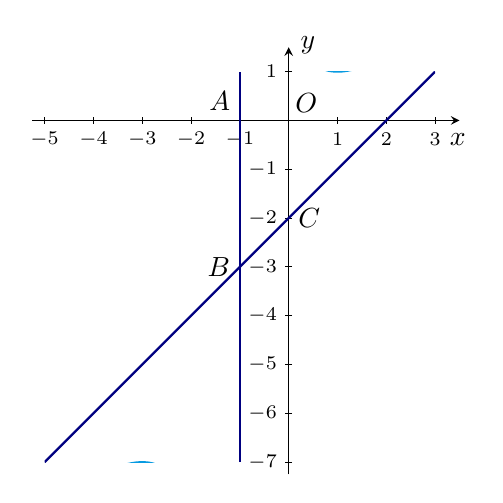
\begin{tikzpicture}[line cap=butt,line join=miter,>=stealth,xscale=0.62,yscale=0.62]
				\tikzset{declare function={xmin=-5;xmax=3;Xkxd=-1;
						ymin=-7;ymax=1;
						a=1; b=-1; c=2; d=1;et=1;
						akxd=1;bkxd=-2;
						f(\x)=(a*(\x)^2+b*\x+c)/(d*(\x)+et);
						h(\x)=akxd*\x+bkxd;
					},
					smooth,samples=50
				}
				\draw[->] (xmin-0.25,0)--(xmax+0.5,0)
				node[shift={(-95:7pt)},font=\normalsize]{$ x $};
				\draw[->] (0,ymin-0.25)--(0,ymax+0.5)
				node[shift={(5:7pt)},font=\normalsize]{$ y $};
				\fill (0,0) node[shift={(45:9pt)},font=\normalsize]{$ O $};
				\foreach \x in {-5, -4, -3, -2, -1, 1, 2, 3}{
					\draw (\x,2pt)--(\x,-2pt) +(0,-9pt) node[font=\scriptsize,fill=white,inner sep=1pt]{$\x$};
				}
				\foreach \y in {-7, -6, -5, -4, -3, -2, -1, 1}{
					\draw (2pt,\y)--(-2pt,\y) +(-3pt,0) node[font=\scriptsize,anchor=east,fill=white,inner sep=1pt]{$\y$};
				}
				\begin{scope}[thick]
					\clip (xmin,ymin) rectangle (xmax,ymax);
					\draw[blue!50!black] (Xkxd,ymin)--(Xkxd,ymax);
					\draw[blue!50!black] plot[domain=xmin:xmax] (\x, {h(\x)});
					\draw[cyan!85!blue] plot[domain=xmin:{Xkxd-0.01}] (\x, {f(\x)});
					\draw[cyan!85!blue] plot[domain={Xkxd+0.01}:xmax] (\x, {f(\x)});
				\end{scope}
				\node [left] at (-1,-3) {$B$}; 
				\node [ above left] at (-1,0) {$A$};
				\node [right] at (0,-2) {$C$};  
			\end{tikzpicture}
		\end{center}
		Tứ giác cần tìm là hình thang vuông $OABC$, ta có $S_{OABC}=\dfrac{(OC+AB)\cdot OA}{2}=\dfrac{5\cdot 2}{2}=5$.
	\end{itemchoice}}
\end{ex}
\begin{ex}%Câu 2
	Một con sư tử đang đuổi theo một con ngựa vằn. Con ngựa vằn nhận ra con sư tử khi con sư tử cách xa nó $40$ m. Từ thời điểm này, con sư tử đuổi con ngựa vằn với tốc độ $v_1(t)=15\mathrm{e}^{-0{,}1t}$ m/s và con ngựa vằn chạy trốn với tốc độ $v_2(t)=20-20\mathrm{e}^{-0{,}1t}$ m/s trên cùng một đường thẳng (với $t$ tính theo giây và $0\le t\le 60$). Xét tính đúng sai của các mệnh đề sau
	\choiceTF
	{Tại thời điểm $t=0$ vận tốc của con ngựa vằn là $20$ m/s}
	{\True Tốc độ của sư tử giảm dần theo thời gian trong khi tốc độ của ngựa vằn tăng dần theo thời gian}
	{Sư tử sẽ ở gần với ngựa vằn nhất khi $v'_1(t)=v'_2(t)$}
	{Sư tử sẽ không bắt được con ngựa vằn và khoảng cách ngắn nhất giữa chúng là $1{,}42$ mét (kết quả làm tròn đến hàng phần trăm)}
	\loigiai{
	\begin{itemchoice}
		\itemch \textbf{Sai.}\\
		Tại $t=0$, ta có $v_2(0)=20-20=0$ m/s.
		\itemch \textbf{Đúng.}\\
		Ta có $v'_1(t)=-0{,}1\cdot 15\mathrm{e}^{-0{,}1t}<0$, $\forall 0\le t\le 60$. Do đó, tốc độ của sử tử giảm dần theo thời gian.\\
		Lại có $v'_2(t)=0{,}1\cdot 20\mathrm{e}^{-0{,}1t}>0$, $\forall 0\le t\le 60$. Do đó, tốc độ của ngựa vằn tăng dần theo thời gian.
		\itemch \textbf{Sai.}\\
		Ta có $v'_1(t)=v'_2(t)\Leftrightarrow 15\mathrm{e}^{-0{,}1t}=-20\mathrm{e}^{-0{,}1t}$. Phương trình này vô nghiệm.
		\itemch \textbf{Sai.}\\
		Chọn hệ quy chiếu với gốc của chuyển động ở vị trí con sư tử bắt đầu đuổi con ngựa vằn.\\
		Gọi $s_1(t)$ là quãng đường con sư tử di chuyển được trong $t$ giây, $s_2(t)$ là quãng đường con ngựa vằn di chuyển được trong $t$ giây.\\
		Ta có $s_1(t)=\displaystyle\int v_1(t)\mathrm{\,d}t=-150\mathrm{e}^{-0{,}1t}+C$.\\
		Tại $t=0$, ta có $s_1(0)=0\Leftrightarrow -150+C=0\Leftrightarrow C=150$. Do đó, $s_2(t)=-150\mathrm{e}^{-0{,}1t}+150$.\\
		Ta có $s_2(t)=\displaystyle\int v_2(t)\mathrm{\,d}t=20t+200\mathrm{e}^{-0{,}1t}+C$.\\
		Tại $t=0$, ta có $s_2(0)=40\Leftrightarrow 200+C=40\Leftrightarrow C=-160$. Do đó, $s_1(t)=20t+200\mathrm{e}^{-0{,}1t}-160$.\\
		Sư tử sẽ ở gần ngựa vằn nhất khi $s_2(t)-s_1(t)$ đạt $\min$. Ta có
		\[s_2(t)-s_1(t)=f(t)=20t+350\mathrm{e}^{-0{,}1t}-310,\forall 0\le t\le 60.\]
		Lại có $f'(t)=20-35\mathrm{e}^{-0{,}1t}$, $\forall 0\le t\le 60$. Khi đó, $f'(t)=0\Leftrightarrow \mathrm{e}^{-0{,}1t}=\dfrac{4}{7}\Leftrightarrow t\approx 5{,}6$ s.\\
		Ta có bảng biến thiên
		\begin{center}
			
\begin{tikzpicture}
			\tkzTabInit[nocadre=false,lgt=1.2,espcl=2.5,deltacl=0.6]
			{$t$/0.6,$f'(t) $/0.6,$f(t)$/2}
			{$0$,$5{,}6$,$60$}
			\tkzTabLine{,-,0,+,} %
			\tkzTabVar{+/$40$,-/$1{,}92$, +/$890{,}1$} %dấu mũi tên, + trên, -dưới
		\end{tikzpicture}
		\end{center}
		Vậy khoảng cách ngắn nhất là $1{,}92$ m.
	\end{itemchoice}}
\end{ex}
\renewcommand{\baselinestretch}{1.5}
\begin{ex}%Câu 3
	Một vật dụng bằng sắt đang nằm trên mặt sàn có tay cầm dài $58$ cm nối với một ống trụ dày $4$ cm và có đường kính đáy bằng $30$ cm. Nếu không giữ thì sẽ luôn có một lực làm vật rung động, để vật đứng yên thì người ta đã nối một đoạn dây từ điểm $B$ (là một điểm nằm trên đường tròn chính giữa của ống trụ to) đến điểm $C$ nằm trên bờ tường. Trên hệ trục $Oxyz$, xét gốc tọa độ là điểm gắn ống trụ với bờ tường, bờ tường là mặt phẳng $(Oxz)$, trục $Oy$ là trục của hình trụ, điểm $A$ nằm chính giữa ống trụ to, điểm $B$ có hoành độ âm, cao độ dương và $AB$ tạo với trục $Oz$ một góc $30^\circ$, các số liệu được cho như hình vẽ, đơn vị trên các hệ trục tính theo cm. Biết rằng lực căng $\overrightarrow{T}$ trên đoạn dây $BC$ có độ lớn bằng $500$ N. Xét tính đúng sai của các mệnh đề sau
	\begin{center}
		\begin{tikzpicture}[scale=1,>=stealth, font=\footnotesize, line join=round, line cap=round]
			\fill[gray!20] (-0.58,-0.85)--(-0.58,3.38)--(4.01,5.22)--(4.01,0.98)--cycle;
			\coordinate (O) at (0,0);
			\coordinate (y) at (5.27,-2.17);
			\coordinate (x) at (4.48,1.79);
			\coordinate (A) at ($(O)!0.7!(y)$);
			\coordinate (E) at (2.75,-0.9);
			\path 
			
			;
			\tkzDefLine[parallel=through E](O,y) \tkzGetPoint{d}
			\tkzInterLL(O,x)(E,d)\tkzGetPoint{E'}
			\draw (E)--(E');
			\coordinate (F) at (2.6,-1.3);
			\tkzDefLine[parallel=through F](O,y) \tkzGetPoint{d'}
			\tkzInterLL(O,x)(F,d')\tkzGetPoint{F'}
			\draw (F)--(F');
			\fill[gray!40] (E)--(E')--(E')..controls+(150:0.5) and +(50:0.1)..(F')--(F)--cycle;
			\begin{scope}[rotate=-20]
				\draw[fill=gray!80] (A) ellipse (0.8 cm and 1.38 cm);
				\coordinate (M) at ($(A)+(90:0.8 cm and 1.38 cm)$);
				\coordinate (M') at ($(M)+(-0.3,0)$);
				\coordinate (N) at ($(A)+(-90:0.8 cm and 1.38 cm)$);
				\coordinate (N') at ($(N)+(-0.3,0)$);
				\draw (M)--(M');
				\draw (N)--(N');
				\draw (M') arc(90:270:0.8 cm and 1.38 cm);
				\fill[gray!40] (M)--(M') arc(90:270:0.8 cm and 1.38 cm)--(N)--(N) arc(270:90:0.8 cm and 1.38 cm)--cycle;
			\end{scope}
			\coordinate (B) at (3.05,-0.7);
			\coordinate (C) at (2.58,3.7);
			\coordinate (I) at ($(A)+(0,2)$);
			\fill (B)node[above left]{$B$}circle(2pt);
			\draw (1.64,-2.21)--(A)--(B) (0.26,-1.33)node[below left]{$60$ cm} (5,-1.29)node[below right]{$15$ cm} (4.47,-0.31)--(5.56,-0.76) ($(B)!0.7!(C)$)--(C)--($(C)+(0,0.5)$) (1.27,3.64)node[above]{$35$ cm} (C)--(3.84,4.21) (3.39,2.69)node[right]{$30$ cm} ($(B)!0.5!(C)$)node[left]{$\overrightarrow{T}$} (A)--(I);
			\draw[->,dashed] (-1.88,-0.75)--(4.48,1.79)node[below]{$x$};
			\draw[->,dashed] (O)node[below left,xshift=0.2cm,yshift=-0.1cm]{$O$}--(0,4)node[right]{$z$};
			\draw[->,dashed] (O)--(y)node[below]{$y$};
			\fill (O)circle(2pt);
			\fill (A)node[above right]{$A$}circle(2pt);
			\fill (C)node[above right,yshift=0.1cm]{$C$}circle(2pt);
			\draw[<->] (-1.51,-0.6)--(2.02,-2.06);
			\draw[<->] (4.7,-1.94)--(5.3,-0.65);
			\draw[<->] (0,3.12)--(2.58,4.16);
			\draw[<->] (3.39,4.03)--(3.39,1.36);
			\draw[->] (B)--($(B)!0.7!(C)$);
			\draw pic[draw,,angle radius=4mm]{angle=I--A--B};
			\draw pic["$30^\circ$",-stealth,angle radius=11mm]{angle=I--A--B};
		\end{tikzpicture}
	\end{center}
	\choiceTF
	{\True Hình chiếu của $C$ lên mặt phẳng $(Oxy)$ có tọa độ $(35;0;0)$}
	{Góc giữa đường thẳng $AB$ và mặt phẳng $(Oxy)$ bằng $30^\circ$}
	{Vectơ $\overrightarrow{BC}$ có tọa độ $(a;b;c)$. Khi đó $2a-b=40$}
	{Vectơ lực tác dụng lên đoạn dây $BC$ có hoành độ là $120$ (làm tròn kết quả đến hàng đơn vị theo Newton)}
	\loigiai{
	\begin{itemchoice}
		\itemch \textbf{Đúng.}\\
		Điểm $C$ có tọa độ $(35;0;30)$ nên hình chiếu của $C$ lên mặt phẳng $(Oxy)$ có tọa độ $(35;0;0)$.
		\itemch \textbf{Sai.}\\
		Ta có $(AB;Oz)=30^\circ$ mà $Oz\perp (Oxy)$ nên $(AB;(Oxy))=60^\circ$.
		\itemch \textbf{Sai.}\\
		Vì đường kính đáy bằng $30$ nên bán kính đáy bằng $15$.\\
		Ta có $|x_B|=AB\cdot\cos 60^\circ=7{,}5$. Mà $x_B<0$ nên $x_B=-7{,}5$.\\
		Lại có $|z_B|=AB\cdot \cos 30^\circ=\dfrac{15\sqrt{3}}{2}$ mà $z_B>0$ nên $z_B=\dfrac{15\sqrt{3}}{2}$. Do đó, $B=\left(-7{,}5;60;\dfrac{15\sqrt{3}}{2}\right)$.
		Khi đó, $\overrightarrow{BC}=\left(42{,}5;-60;30-\dfrac{15\sqrt{3}}{2}\right)$. Suy ra $2a-b=2\cdot42{,}5+60=145$.
		\itemch \textbf{Sai.}\\
		Ta có $\left|\overrightarrow{BC}\right|=\sqrt{(42{,}5)^2+60^2+\left(30-\dfrac{15\sqrt{3}}{2}\right)}\approx 75$.\\
		Suy ra $\overrightarrow{T}=\dfrac{500}{75}\overrightarrow{BC}$ nên hoành độ của $\overrightarrow{T}$ bằng $\dfrac{500}{75}\cdot 42{,}5\approx 283$.
	\end{itemchoice}}
\end{ex}
\begin{ex}%Câu 4
	Trong một khu dân cư, tỉ lệ người nghiện thuốc lá và và bị ung thư vòm họng là $15\%$. Có $25\%$ người nghiện thuốc lá nhưng không bị ung thư vòm họng, $50\%$ người không nghiện thuốc lá và không bị ung thư họng và có $10\%$ số người không nghiện thuốc lá nhưng mắc ung thư vòm họng.
	\begin{itemize}
		\item Gọi $A$ là biến cố \lq\lq người đó nghiện thuốc lá\rq\rq.
		\item Gọi $B$ là biến cố \lq\lq người đó bị ung thư vòm họng\rq\rq.
	\end{itemize}
	Xét tính đúng sai của các mệnh đề sau
	\choiceTF
	{$\mathrm{P}(AB)=0{,}25$ và $\mathrm{P}(\overline{A}B)=0{,}15$}
	{$\mathrm{P}(A)=0{,}6$}
	{\True $\mathrm{P}(B\mid A)=0{,}375$}
	{\True Với những dữ liệu thống kê như trên có thể thấy nguy cơ của người nghiện thuốc là mắc ung thư vòm họng gấp $2{,}25$ lần người không nghiện thuốc lá}
	\loigiai{
	\begin{itemchoice}
		\itemch \textbf{Sai.}\\
		Ta có $\mathrm{P}(AB)=0{,}15$, $\mathrm{P}(\overline{A}B)=0{,}1$.
		\itemch \textbf{Sai.}\\
		Ta có $\mathrm{P}(A)=\mathrm{P}(AB)+\mathrm{P}(A\overline{B})$.\\
		Theo đề, ta có $\mathrm{P}(A\overline{B})=0{,}25$, $\mathrm{P}(\overline{A}\cap\overline{B})=0{,}5$, $\mathrm{P}(\overline{A}B)=0{,}1$.\\
		Do đó, $\mathrm{P}(A)=0{,}15+0{,}25=0{,}4$.
		\itemch \textbf{Đúng.}\\
		Ta có $\mathrm{P}(B\mid A)=\dfrac{\mathrm{P}(AB)}{\mathrm{P}(A)}=\dfrac{0{,}15}{0{,}4}=0{,}375$.
		\itemch \textbf{Đúng.}\\
		Ta có $\mathrm{P}(B\mid \overline{A})=\dfrac{\mathrm{P}(B\overline{A})}{\mathrm{P}(\overline{A})}=\dfrac{0{,}1}{0{,}6}=\dfrac{1}{6}$.\\
		Do đó $\mathrm{P}(B\mid A)=2{,}25\cdot\mathrm{P}(B\mid\overline{A})$.
	\end{itemchoice}}
\end{ex}
\Closesolutionfile{ans}
\TNSA
% \setcounter{ex}{0}% Reset lại số đếm câu hỏi
\Opensolutionfile{ans}[ans/de3-phanIII]
\begin{ex}%Câu 1
	Cho hình chóp $S.ABC$ có cạnh bên $SA$ vuông góc với mặt phẳng $(ABC)$ và $AB=1$, $AC=2$, $\widehat{BAC}=60^\circ$. Khoảng cách giữa hai đường thẳng $SA$ và $BC$ bằng bao nhiêu?
	
	\shortans[]{$1$}
	\loigiai{
	\begin{center}
		\begin{tikzpicture}
		\def\a{4} %Khai báo cạnh
		\def\h{4}
		\path 	(0:0) coordinate (A)
		++(0:\a) coordinate (C)
		++(-150:4*\a/5) coordinate (B)
		($(A)+(90:\h)$) coordinate (S)
		($(B)!0.3!(C)$) coordinate (H);
		\draw[thick] 	(A)--(B)--(C)
		(A)--(S)--(H)	(C)--(S)	(B)--(S);
		\draw[dashed,thick] 	(H)--(A)--(C);
		\foreach \x /\goc in {A/180,C/0,B/-135,S/90,H/-45}
		\fill[black] (\x) circle (1.5pt)
		($(\x)+(\goc:3mm)$) node {$\x$};
		\draw pic[draw,angle radius=2mm]{right angle=C--A--S};%Theo chiều dương
		\draw pic[draw,angle radius=2mm]{right angle=A--H--C};
		\end{tikzpicture}
		\end{center}
	Kẻ $AH\perp BC$ ($H\in BC$).\\
	Ta có $SA\perp(ABC)$ nên $SA\perp AH$. Do đó, $AH$ là đoạn vuông góc chung của $SA$ và $BC$.\\
	Suy ra $\mathrm{d}(SA,BC)=AH$.\\
	Lại có $BC=\sqrt{AB^2+AC^2-2AB\cdot AC\cdot \cos \widehat{BAC}}=\sqrt{1+4-2\cdot1\cdot2\cdot\cos 60^\circ}=\sqrt{3}$.\\
	Mà $S_{ABC}=\dfrac{1}{2}AH\cdot BC=\dfrac{1}{2}AB\cdot AC\sin\widehat{BAC}$ nên $AH=\dfrac{AB\cdot AC\sin\widehat{BAC}}{BC}=1$.}
\end{ex}
\begin{ex}%Câu 2
	Trong một vườn cây ăn trái, có ba loại cây: cây cam, cây chanh và cây bưởi. Sau $3$ năm, số cây cam tăng gấp ba lần, số cây chanh tăng gấp hai lần và cây bưởi tăng gấp bốn lần số lượng cây ban đầu. Tổng số cây sau $3$ năm là $330$ cây. Biết rằng ban đầu số lượng cây bưởi bằng trung bình cộng của số lượng cây cam và cây chanh. Sau $3$ năm thu hoạch, tổng số cây cam và cây chanh tăng thêm nhiều hơn $15$ cây so với số cây bưởi tăng thêm. Vậy tổng số cây cam và cây bưởi ban đầu là bao nhiêu?
	
	\shortans[]{$85$}
	\loigiai{
	Gọi $x$ (cây) là số cây cam ban đầu, $y$ (cây) là số cây bưởi ban đầu, $z$ (cây) là số cây chanh ban đầu.\\
	Theo đề, ta có $\heva{&3x+4y+2z=330 \\&y=\dfrac{x+z}{2} \\&2x+z-3y=15}\Leftrightarrow\heva{&x=50 \\&y=35 \\&z=20.}$\\
	Vậy tổng số cây cam và cây bưởi ban đầu là $50+35=85$ cây.}
\end{ex}
\begin{ex}%Câu 3
	Có hai bình như sau: Bình $A$ chứa $5$ bi đỏ, $3$ bi trắng và $8$ bi xanh; bình $B$ chứa $3$ bi đỏ và $5$ bi trắng. Gieo một con xúc xắc ngẫu nhiên: Nếu mặt $3$ hoặc mặt $5$ xuất hiện thì chọn ngẫu nhiên một bi từ bình $B$; các trường hợp khác thì chọn ngẫu nhiên một bi từ bình $A$. Nếu viên bi trắng được chọn ra, hãy tính xác suất để mặt $5$ của con xúc xắc xuất hiện nhiều nhất.
	
	\shortans[]{$0{,}31$}
	\loigiai{
	Gọi $A$ là biến cố \lq\lq Bi được chọn là bi trắng\rq\rq, $B$ là biến cố \lq\lq Xúc xắc xuất hiện mặt 5\rq\rq.\\
	Ta cần tính $\mathrm{P}(B\mid A)$. Theo công thức xác suất Bayes, ta có $\mathrm{P}(B\mid A)=\dfrac{\mathrm{P}(B)\cdot\mathrm{P}(A\mid B)}{\mathrm{P}(A)}$.\\
	Theo đề, ta có $\mathrm{P}(B)=\dfrac{1}{6}$, $\mathrm{P}(A\mid B)=\dfrac{5}{8}$.\\
	Lại có $\mathrm{P}(A)=\mathrm{P}(AB)+\mathrm{P}(A\overline{B})$.\\
	Nếu xúc xắc đổ ra số $3$, khi đó xác suất bốc trúng bi trắng là $\dfrac{5}{8}$.\\
	Nếu xúc xắc đổ ra các số còn lại (ngoại trừ số $5$) thì xác suất bốc trúng bi trắng là $\dfrac{3}{16}$.\\
	Do đó, $\mathrm{P}(A\overline{B})=\dfrac{1}{6}\cdot\dfrac{5}{8}+\dfrac{2}{3}\cdot\dfrac{3}{16}=\dfrac{11}{48}$. Suy ra $\mathrm{P}(A)=\dfrac{1}{6}\cdot\dfrac{5}{8}+\dfrac{11}{48}=\dfrac{1}{3}$.\\
	Vậy $\mathrm{P}(B\mid A)=\dfrac{\dfrac{1}{6}\cdot\dfrac{5}{8}}{\dfrac{1}{3}}=\dfrac{5}{16}=0{,}3125$.
	}
\end{ex}
\begin{ex}%Câu 4
	Cần trục chân đế là kiểu cột quay được sử dụng để phục vụ công việc xếp dỡ hàng hóa chủ yếu ngoài các cảng, bến, bãi (như hình minh họa).
	
	{\centering \begin{tikzpicture}[scale=0.7,>=stealth, font=\footnotesize, line join=round, line cap=round]
			\draw (0,0)node[opacity=0.65]{\includegraphics[scale=0.21]{images/de3-1}};
			\coordinate (K) at (1.85,1.3);
			\coordinate (M) at (-3,2.9);
			\coordinate (O) at (2.75,-3.15);
			\fill (K)node[above right,font=\bfseries]{$K$}circle(3pt);
			\fill (M)node[above,font=\bfseries]{$M$}circle(3pt);
			\draw[->,thick] (O)--($(O)!1.4!(K)$)node[right,font=\bfseries]{$z$};
			\draw[->,thick] (O)--(3.7,-2.85)node[above,font=\bfseries]{$x$};
			\draw[->,thick] (O)--($(O)+(-6.5,0)$)node[above,font=\bfseries]{$y$};
	\end{tikzpicture}\par}\noindent
	Ta chọn hệ trục $Oxyz$ thỏa mãn $(Oxy)$ song song với mặt đất, trục $Ox$ trùng với trục chân đế, trục $Oz$ trùng với trục cần cẩu và trục $Oy$ như hình vẽ. Gọi $M$ là vị trí tại đỉnh cần cẩu, $H$ là hình chiếu của $M$ lên $(Oxy)$. Biết tay cần $KM$ của cần trục dài $50$ m, trục cần $OK$ dài $50$ m, $\left(\overrightarrow{k},\overrightarrow{KM}\right)=60^\circ$; $\left(\overrightarrow{i},\overrightarrow{OH}\right)=45^\circ$. Biết điểm $M$ có tọa độ $M(a;b;c)$ trong hệ tọa độ $Oxyz$ trên, giá trị của $a+b+c$ bằng bao nhiêu? (làm tròn kết quả đến hàng đơn vị).
	
	\shortans[]{$136$}
	\loigiai{
	Theo đề, ta có $c=OK+KM\cdot\cos 60^\circ=\dfrac{50}{2}=75$, $a=x_H$, $b=y_H$.\\
	Vì $\left(\overrightarrow{i},\overrightarrow{OH}\right)=45^\circ$ và $OH=MK\cdot\sin 60^\circ=25\sqrt{3}$ nên $x_H=y_H=\dfrac{OH}{\sqrt{2}}=\dfrac{25\sqrt{3}}{\sqrt{2}}$.\\
	Vậy $M\left(\dfrac{25\sqrt{3}}{\sqrt{2}};\dfrac{25\sqrt{3}}{\sqrt{2}};75\right)$ nên $a+b+c=25\sqrt{6}+75\approx 136$.}
\end{ex}
\begin{ex}%Câu 5
	\immini[thm]
	{
		Hai hình chữ nhật bằng nhau, nội tiếp trong đường tròn tâm $O$, bán kính $r=1$ cm tạo thành một hình chữ thập đối xứng (như hình vẽ bên). Diện tích lớn nhất của hình chữ thập là bao nhiêu cm$^2$? (Kết quả làm tròn đến hàng phần trăm).
		
	\shortans[]{$2{,}47$}
	}
	{
		\begin{tikzpicture}[scale=0.8,>=stealth, font=\footnotesize, line join=round, line cap=round]
			\coordinate (O) at (0,0);
			\coordinate (A) at (-1,2);
			\coordinate (B) at (1,2);
			\coordinate (C) at (1,1);
			\coordinate (D) at (2,1);
			\coordinate (E) at (2,-1);
			\coordinate (F) at (1,-1);
			\coordinate (G) at (1,-2);
			\coordinate (H) at (-1,-2);
			\coordinate (I) at (-1,-1);
			\coordinate (J) at (-2,-1);
			\coordinate (K) at (-2,1);
			\coordinate (L) at (-1,1);
			\draw (O) circle(2.236 cm);
			\draw (A)--(B)--(C)--(D)--(E)--(F)--(G)--(H)--(I)--(J)--(K)--(L)--cycle;
			\fill[color=gray!80,opacity=0.5pt] (A)--(B)--(C)--(D)--(E)--(F)--(G)--(H)--(I)--(J)--(K)--(L)--cycle;
			\draw (O)--(D) ($(O)!0.5!(D)$)node[below]{$r$};
			\fill (O)node[below]{$O$}circle(2pt);
			
		\end{tikzpicture}
	}
	\loigiai{
	\begin{center}
		\begin{tikzpicture}[scale=0.8,>=stealth, font=\footnotesize, line join=round, line cap=round]
		\coordinate (O) at (0,0);
		\coordinate (A) at (-1,2);
		\coordinate (B) at (1,2);
		\coordinate (C) at (1,1);
		\coordinate (D) at (2,1);
		\coordinate (E) at (2,-1);
		\coordinate (F) at (1,-1);
		\coordinate (G) at (1,-2);
		\coordinate (H) at (-1,-2);
		\coordinate (I) at (-1,-1);
		\coordinate (J) at (-2,-1);
		\coordinate (K) at (-2,1);
		\coordinate (L) at (-1,1);
		\draw (O) circle(2.236 cm);
		\draw (A)--(B)--(C)--(D)--(E)--(F)--(G)--(H)--(I)--(J)--(K)--(L)--cycle;
		\fill[color=gray!80,opacity=0.5pt] (A)--(B)--(C)--(D)--(E)--(F)--(G)--(H)--(I)--(J)--(K)--(L)--cycle;
		\draw (O)--(D) ($(O)!0.5!(D)$)node[left]{$r$};
		\fill (O)node[below]{$O$}circle(2pt);
		\foreach \x /\goc in {A/160,C/45,B/45,D/0,E/-45,F/-45,I/-135,G/-30,H/-120,J/180,K/180,L/135}
		\fill[black] (\x) circle (1.5pt)
		($(\x)+(\goc:3mm)$) node {$\x$};
		\draw[dashed] (O)--(2,0) (L)--(C)--(F)--(I)--cycle;
	\end{tikzpicture}
	\end{center}
	Đặt $DE=AB=KJ=HG=x$ (cm). Ta có $\dfrac{JE}{2}=\sqrt{1-\dfrac{x^2}{4}}\Rightarrow JE=\sqrt{4-x^2}$.\\
	Khi đó, diện tích hình chữ thập bằng \[S_{KDEJ}+2S_{ABCL}=x\sqrt{4-x^2}+x\left(\sqrt{4-x^2}-x\right)=-x^2+2x\sqrt{4-x^2}.\]
	Xét $f(x)=-x^2+2x\sqrt{4-x^2}$, với $0<x<2$.\\
	Ta có $f'(x)=-2x+2\sqrt{4-x^2}-\dfrac{2x^2}{\sqrt{4-x^2}}$, với $0<x<2$.\\
	Khi đó $f'(x)=0\Leftrightarrow x+\dfrac{x^2}{\sqrt{4-x^2}}=\sqrt{4-x^2}\Leftrightarrow x\sqrt{4-x^2}=4-2x^2\Leftrightarrow x\approx1{,}05$.\\
	Do đó, $\displaystyle\max_{(0;2)}f(x)=f(1{,}05)\approx 2{,}47$.
	}
\end{ex}
\begin{ex}%[1H8V7-9]%[TEX ĐỀ MOON 2025]%[Huỳnh Thanh Chí]
	Người ta cần trang trí một kim tự tháp hình chóp tứ giác đều $S.ABCD$ có cạnh bên bằng $200$ m, góc $\widehat{ASB}=15^\circ$ bằng đường gấp khúc dây đèn led vong quanh kim tự tháp $AEFGHIJKLS$. Trong đó điểm $L$ cố định và $LS=40$ m.
	\begin{center}
		\begin{tikzpicture}[scale=1,>=stealth, font=\footnotesize, line join=round, line cap=round]
			\coordinate (A) at (-1.9,-1.6);
			\coordinate (B) at (0,0);
			\coordinate (D) at (1.6,-1.6);
			\coordinate (C) at ($(B)+(D)-(A)$);
			\coordinate (O) at ($(A)!1/2!(C)$);
			\coordinate (S) at ($(O)+(0,4)$);
			\coordinate (L) at ($(S)!0.2!(A)$);
			\coordinate (K) at ($(S)!0.28!(D)$);
			\coordinate (J) at ($(S)!0.4!(C)$);
			\coordinate (I) at ($(S)!0.65!(B)$);
			\coordinate (H) at ($(S)!0.45!(A)$);
			\coordinate (G) at ($(S)!0.55!(D)$);
			\coordinate (F) at ($(S)!0.7!(C)$);
			\coordinate (E) at ($(S)!0.8!(B)$);
			\draw (S)--(A)--(D)--(C)--cycle (S)--(D) (F)--(G)--(H) (J)--(K)--(L);
			\draw[dashed] (A)--(B)--(C) (S)--(B) (A)--(E)--(F) (H)--(I)--(J);
			\foreach \x/\g in {S/90,A/-150,B/-60,C/0,D/-45,E/170,F/45,G/-30,H/170,I/140,J/30,K/60,L/170}
			\fill[black] (\x) circle (1pt) ($(\g:3mm)+(\x)$) node {$\x$};
		\end{tikzpicture}
	\end{center}
	Hỏi khi đó cần dùng ít nhất bao nhiêu mét dây đèn led để trăng trí? (làm tròn đến hàng đơn vị).
	
	\shortans[]{$263$}
	\loigiai{
		Ta trải hình chóp tứ giác đều thành vẽ như sau
		\begin{center}
			\begin{tikzpicture}[scale=1.5,font=\footnotesize,line join=round,line cap=round,>=stealth]
				\def\a{4}
				\def\r{15}
				\path 
				(0,0) coordinate (S)
				(-135:\a) coordinate (A)
				(-135+\r:\a) coordinate (D)
				($(A)!1!-90:(D)$) coordinate (B_2)
				($(D)!1!90:(A)$) coordinate (C_2)
				;
				\foreach \x/\i in {C/2,B/3,A_1/4,D_1/5,C_1/6,B_1/7,A_2/8}{
					\path 
					(-135+\i*\r:\a) coordinate (\x)
					;
					\draw (S)--(\x);	
				}
				\foreach \x/\y/\i in {A/L/1,D/K/2,C/J/3,B/I/4,A_1/H/5,D_1/G/6,C_1/F/7,B_1/E/8,
					A_1/H_1/7,B/I_1/6,C/J_1/5,D/K_1/4
				}{
					\path 
					($(S)!1/9*\i!(\x)$) coordinate (\y)
					;}
				\draw (S)--(D)--(C_2)--(B_2)--(A)--(S) (A)--(D)--(C)--(B)--(A_1)--(D_1)--(C_1)--(B_1)--(A_2)
				(L)--(K)--(J)--(I)--(H)--(G)--(F)--(E)--(A_2)--(L)
				%	(K1)--(J1)--(I1)--(H1)
				;
				
				\foreach \x/\g in {A/135,D/-65,S/180,C/-90,B/-90,A_1/-90,D_1/-90,C_1/-60,B_1/-45,A_2/0,C_2/-135,B_2/-90}
				\fill 	(\x) circle (1pt)
				($(\g:3mm)+(\x)$) node {$\x$};
				\foreach \x/\g in {L/135,K/-90,J/-90,I/-90,H/-90,G/-90,F/-90,E/-90}
				\fill 	(\x) circle (1pt)
				($(\g:3mm)+(\x)$) node {$\x$};
			\end{tikzpicture}
		\end{center}
		Ta có $T=SL+LK+KJ+\ldots+EA_2\ge SL+LA_2$ (vì $SL$ không đổi).\\
		Để sợi dây trang trí ngắn nhất thì $T=SL+LA_2$.\\
		Ta có $\widehat{LSA_2}=15^\circ \cdot 8=120^\circ$.\\
		Áp dụng định lí cosin vào $\triangle SLA_2$ có
		\allowdisplaybreaks
		\begin{eqnarray*}
			LA_2=\sqrt{SL^2+SA_2^2-2\cdot SL\cdot SA_2\cdot\cos \widehat{SLA_2}}=40\sqrt{31}.
		\end{eqnarray*}
		Vậy $T=40+40\sqrt{31}\approx 263$.
	}
\end{ex}
\Closesolutionfile{ans}